\documentclass[letterpaper]{article}

\usepackage{graphicx}
\usepackage[parfill]{parskip}
\usepackage{setspace}
\usepackage{amsfonts}
\usepackage{amsmath}
\usepackage{amssymb}

\newcommand{\Rationals}{\mathbb{Q}}
\newcommand{\Integers}{\mathbb{Z}}
\newcommand{\Naturals}{\mathbb{N}}

\begin{document}
\noindent{\Large\textbf{M311S24 Problem Set 3} \textit{Franchi-Pereira, Philip}} \\
\begin{itemize}
    \item[\textbf{Problem 1}] Extend the Chinese Remainder Theorem to find the solutions in \(\Integers_{210}\) of the following equations.
          \begin{center}
              \begin{tabular}{ p{3cm} p{3cm} p{3cm} }
                  \(2x \equiv_{7} 3 \) & \(x \equiv_{5} 4\) & \(3x \equiv_{6} 3\)
              \end{tabular}
          \end{center}

          \textbf{Solution:} To start, we simplify the first equation to isolate \(x\) by multiplying both sides by \(2^-1\) to get \(x \equiv_{7} 5 \). Then we compute the solutions to \(x \equiv_{7} 5 \) and \(x \equiv_{5} 4\). Using the extended Euclidean algorithm, we get that \((7,5) = 1\), with values for \(\lambda = -2\) and \(\omega = 3\) \(-2\cdot 7 + 3\cdot 5 = 1\). So, the solutions to the first twi congruences some multiple of \(5\cdot 15 + 4 \cdot - 14 = 19\) in \(\Integers_{35}\).

          Next, notice that the equation \(3x \equiv_{6} 3\) has three solutions, which by hand we compute to be  \(1, 3\), and \(5\). So we will actually be solving three systems of equations, using the same method: applying the Extended Euclidean Algorithm on (35,6) to find values for \(\lambda\) and \(\omega\), which yield \(\lambda = -1 \) and \(\omega = 6\), then solving \(x = r_{210}( (19 \cdot 6 \cdot 6 )  + (b \cdot 35 \cdot -1 ))\) = \(r_{210}(684 - 35b)\)
          \begin{center}
              \begin{tabular}{ p{2cm}  p{2cm} p{4cm}}
                  \(x \equiv_{35} 19 \)  & \(x \equiv_{6} 1\) & \(r_{210}(684 - 35) = 19\)         \\
                  \(x \equiv_{35} 19  \) & \(x \equiv_{6} 3\) & \(r_{210}(684 - 35\cdot 3) = 159\) \\
                  \(x \equiv_{35} 19  \) & \(x \equiv_{6} 5\) & \(r_{210}(684 - 35\cdot 5) = 89\)
              \end{tabular}
          \end{center}
          So, we have three solutions in \(\Integers_{210},\ 19, 89, 159\).

    \item[\textbf{Problem 2}] Give the divisors and subgroup diagrams for 36.
          \begin{center}

              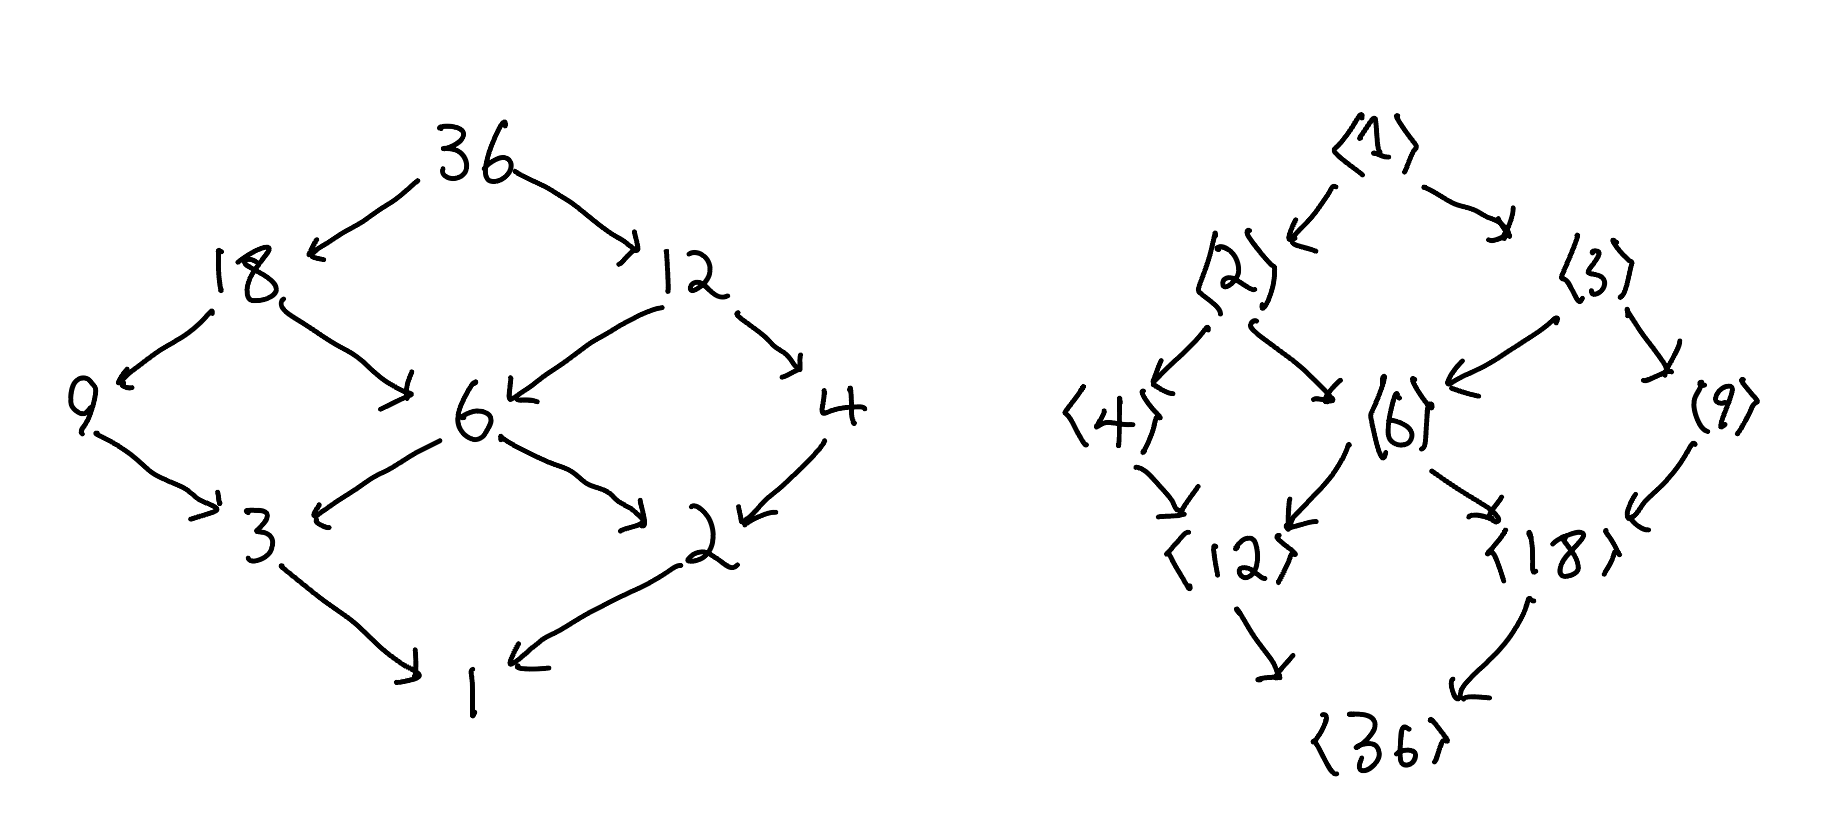
\includegraphics[totalheight=5cm]{images/hw3subgroups.png}
          \end{center}
          \break
    \item[\textbf{Problem 2c}] Give the table of subgroups and generators for 36.
          \begin{center}
              \begin{tabular}{ c | c }
                  group                        & generators                                      \\
                  \hline
                  \(\Integers_{36}\)           & \{1, 5, 7, 11, 13, 17, 19, 23, 25, 29, 31, 35\} \\
                  \(2\Integers_{36}\)          & \{2, 10, 14, 22, 26, 34\}                       \\
                  \(3\Integers_{36}\)          & \{3,15, 21, 33 \}                               \\
                  \(4\Integers_{36}\)          & \{8, 16, 20, 28, 32\}                           \\
                  \(6\Integers_{36}\)          & \{6, 30\}                                       \\
                  \(9\Integers_{36}\)          & \{9, 27\}                                       \\
                  \(12\Integers_{36}\)         & \{12, 24\}                                      \\
                  \(18\Integers_{36}\)         & \{18\}                                          \\
                  \(\{0\} = 36\Integers_{36}\) & \{0\}                                           \\
              \end{tabular}
          \end{center}
    \item[\textbf{Problem 3}] Let \(k \in \Integers_n\). Show that the additive order of \(k\) is \(\frac{n}{(k,n)}\).

          The additive order of \(k\) is defined as an \(m \in \Integers_n\) such that \(m\cdot k \equiv_n 0\).
          Therefore \(n | mk\), and so \(mk = \alpha n\).
          Letting \(d = (k, n)\) we have \(k = h_kd\) and \(n = h_nd\).
          So, \(mh_kd = \alpha h_nd\) and cancelling \(mh_k = \alpha h_n\).
          Since \(h_k | mh_k\) and \(mh_k | \alpha h_n\) we have \(h_k| \alpha h_n\).
          But, \((h_n, h_k) = 1\) so we have \(h_k | \alpha\)
          and \(\alpha = \beta h_k\) for some \(\beta \in \Integers\).
          Therefore \(mh_k = \beta h_k h_n\) and cancelling we have \(m = \beta h_n\).
          So \(m\) is a multiple of \(h_n\), but since it is the smallest positive multiple,W we take \(\beta = 1\) and have \(m = h_n\), which is \(m = \frac{n}{(k,n)}\)
    \item[\textbf{Problem 4a}] Show that \((n-1)! \equiv_n -1\) if \(n\) is prime and \((n-1!) \equiv_n 0\) if \(n\) is composite and \(n > 4\).

          Since \(\Integers_n\) is a commutative ring, every element \(a\) in \(\Integers_n\) except for \(1, n-1,\) and \(0\) have a distinct inverse \(a^{-1}\) such that \(a \cdot a^{-1} = 1\). Since \((n-1)!\) is the product of every integer from 1 to \(n-1\), we have the product \((n-1)! \equiv_n 1\cdot (a_1a_1^{-1})\cdot (a_2a_2^{-1})\cdots (n-1) \equiv_n (1)\cdot{(1)}^{(\frac{n-2}{2})}\cdot(n-1) \equiv_n n-1\).

          If instead \(n\) is composite, then there exist some integers \(a, b\) such that \(n = ab\). We have two cases: either \(a = b\) or \(a \neq b\).
          If \(a \neq b\) then \(ab\) is a product in \((n-1)!\), so \(n | (n-1)!\) and \((n-1)! \equiv_n 0\).

          If instead we have \(a = b\), then \(n = a^2\). If \(a\) is composite, such that \(a = pq\), then we have that \(n = ppqq\), but since \(p\) is a term in \((n-1)!\) and \(pqq\) is a term in \((n-1)!\) then \(ppqq | (n-1)!\).

          Finally, if \(a\) is a prime and \(n = aa\), then \(a\) is clearly a term in \((n-1)!\), but so is \(2a\), when \(n > 4\). Then \(2aa | (n-1)!\), so \((n-1!) \equiv_n 0\).

    \item[\textbf{Problem 4b}]Find \(k \in \Integers_{101}\) such that \(96!\equiv_{101} k\).

          For a prime \(p\), we have shown that \((p-1)! \equiv_{p} p-1\). Observe that for the prime \(p = 101\) the solution to \(96! \equiv_{101} k\) can be found by applying the inverses of \(100, 99, 98, 97\) to the equivalence \(100! \equiv_{101} 1\). Since \(101\) is prime, then the greatest common divisor between it and each of those values is 1. To find the inverses, we note that since \(\lambda n + \omega (101) = 1\), then in \(\Integers_{101},\ \omega (101) = 0 \) and \(\lambda n = 1\), so \(\lambda\) is our inverse. We know the inverse to 100 from Wilson's Theorem, and 3 applications of the Extended Euclidean Algorithm show that:
          \begin{center}
              \begin{tabular}{ p{2cm} p{2cm} p{2cm} p{2cm}}
                  \(100^{-1} = 100\) & \(99^{-1} = 50\) & \(98^{-1} = -34\) & \(97^{-1} = 25\)
              \end{tabular}
          \end{center}
          And so
          \begin{align*}
              (100\cdot 50 \cdot -34 \cdot 25) \cdot (100!)
              \equiv_{101} 96! & \equiv_{101} 100 \cdot (100\cdot 50 \cdot -34 \cdot 25)                   \\
                               & \equiv_{101} 50 \cdot -34 \cdot 25 \equiv_{101} (100) \cdot -17 \cdot 25  \\
                               & \equiv_{101} (100) \cdot -17 \cdot 25 \equiv_{101} (100) \cdot 84\cdot 25
              \\ &\equiv_{101} (100) \cdot 21 \cdot 25 \cdot 4 \equiv_{101} (100) \cdot (100)\cdot 21
              \\ & \equiv_{101} 21
          \end{align*}
          So \(96! \equiv_{101} 21\)
    \item[\textbf{Problem 5}] Compute \(13^{(243^{(65^{35})})}\ (\text{mod } 200)\)

          The factors of \(200\) are \(2^3\cdot 5^2\). Since \(13\) is prime, then \((200, 13) = 1\). By Euler's Theorem, \(13^{\varphi(200)} \equiv_{200} 1\) and we can compute \(\varphi(200) = 200\cdot( 1 - \frac{1}{2})(1 - \frac{1}{5}) = 200 \cdot \frac{4}{10} = 80\). So \(13^{80} \equiv_{200} 1\). Using the division algorithm, we can re-express \(13^{(243^{(65^{35})})}\) as \(13^{k(80) + r} \equiv_{200} (13^{80})^k (13^r) \equiv_{200} (1^k)(13^r) \equiv_{200} 13^r\) for some \(k, r \in \Integers\).

          So to find \(r\), we solve \(243^{(65^{35})} \equiv_{80} r\), and since the prime factors of \(80 = 2^4 \cdot 5\) and \(243 = 3^5\), then applying Euler's theorem again we see that \(\varphi(80)= 32\) and  \(243^{32}\equiv_{80} 1\). So applying the division algorithm again we will find an \(r_2\) such that \(243^{65^{35}} \equiv_{80} 243^{k(32) + r_2}\).

          We must next solve \(65^{35} \equiv_{32} r_2\), and again the factors of \(65 = 13 \cdot 5\) and \(32 = 2^5\), so \(\varphi (32) = 16\) and \(65^{16} \equiv_{32} 1\). Since \(35 = 2\cdot16 + 3\), we have \(65^{35} \equiv_{32} 65^3\), which a calculator shows equals \(274625\) in \(\Integers\).

          Notice next that \(65^{355} \equiv_{32} 274625 \equiv_{32} 1\), so working backwards we have \(r_2 = 1\), so \(243^{65^{35}} \equiv_{80} 243^1\). Then \(r \equiv_{80} 243 \equiv_{80} 3\), so \(13^{(243^{(65^{35})})} \equiv_{200} 35^{243} \equiv_{200} 35^3\), and since \(13^3  = 2197\), we have \(2197 \equiv_{200} 197\).

    \item[\textbf{Problem 6a}] Show that for all primes \(p\), \(n^{k(p-1) + 1} - n \equiv_p 0\).

          Since \(p\) is prime, either \(p\) is a factor of \(n\) or \((n,p) = 1\). If it is a factor, then \(p|n\) and so clearly \(p|n^{k(p-1) + 1}\), so \(n^{k(p-1) + 1} - n \equiv_p 0\)

          If instead \((n,p) = 1\) then we can rewrite \(n^{k(p-1) + 1} - n\) as \(n\cdot n^{k(p-1)} - n\), and since Euler's theorem states that  \(\phi(p) = p-1 \), we have \(n^{k(\phi(p))} \equiv_p n^{(\phi(p))^k} \equiv_p 1\) so the equation becomes \(n\cdot(1^k) - n\) which is \(n-n = 0\) and \(n^{k(p-1) + 1} - n \equiv_p 0\).

    \item[\textbf{Problem 6b}] Show that for all \(n\), \(1919190 | n^{37} - n\).

          By the previous problem, we have \(n^{k(p-1) + 1} - n \equiv_p 0\) for any prime \(p\). We can rewrite \(n^{37} - n = n\cdot n^{36 + 1} - n\), and find factors of \(36\) such that \(k(p-1) = 36\). The values for a prime \(p\) such that \((p-1)|36\) are \(P = \{2, 3, 5, 7, 13, 19, 37\}\). So, for all \(p \in P\) and all \(n \in \Integers\), the congruence \(n^{37} - n \equiv_p 0\) has a solution, and we have \(p | n^{37} - n\). Since every \(p \in P\) is prime, then the product of all \(p \in P\), \(p_1\cdot p_2\cdots p_n | n^{37} - 1\), which is 1919190. Therefore, \(1919190 | n^{37} - n\).

    \item[\textbf{Problem 7}] Show that for all \(n \geq 2,\ 2^n \not\equiv_n  0\).

          Suppose instead that \(2^n \equiv_n 1\). Let \(p\) be the smallest prime factor of \(n\). It is clear that \(n\) must be odd, and so \(p\) must be odd as well. Then by Euler's theorem we have \(2^{(p-1)} \equiv_p 1\) as well as \(2^n \equiv_p = 1\). Then let \(d = (n, p-1)\). If \(d \neq 1\) then we have a contradiction, so \(d = 1\). But then by Bézout's identity we have \(\lambda(p-1) + \omega n = 1\). Observe then that
          \begin{align*}
              2^n \equiv_p 2^{(p-1)}      & \equiv_p {(2^n)}^\omega \equiv_p {(2^{(p-1)})}^\lambda \\
              1\cdot  {(2^n)}^\omega      & \equiv_p {(2^n)}^\omega \cdot {(2^{(p-1)})}^\lambda    \\
              2^{\lambda(p-1) + \omega n} & \equiv_p 2^1 \equiv_p 1
          \end{align*}
          which is a contradiction, since there is no odd prime where \(2 \equiv_p 1\)
\end{itemize}
\end{document}